\documentclass[12pt, fontset=windows]{ctexart}

\usepackage[backend=biber, style=authoryear]{biblatex}
\addbibresource{ref.bib}

\usepackage[margin=1in]{geometry}
\usepackage{graphicx}
\usepackage{booktabs}
\usepackage{array}
\usepackage{longtable}
\usepackage{tabularx}
\usepackage{enumitem}
\usepackage{float}
\usepackage[dvipsnames]{xcolor}
\usepackage[hidelinks]{hyperref}
\usepackage{fancyhdr}
\usepackage{setspace}
\usepackage{titlesec}
\usepackage{tikz}
\usepackage{pgfplots}
\usepackage{amsmath}
\usepackage{amssymb}
\usepackage{caption}
\usetikzlibrary{positioning,arrows.meta,calc,shapes.geometric}
\usepackage{adjustbox}
\usepackage[strings]{underscore}
\usepackage[most]{tcolorbox}
\usepackage{fvextra}
\usepackage{listings}
\usepackage{pdfpages}

 
\definecolor{AquaBlue}{HTML}{1F4E79}
\definecolor{AquaTeal}{HTML}{0B6466}
\definecolor{AquaLight}{HTML}{EEF6FB}
\definecolor{AquaGreen}{HTML}{3A7D44}
\definecolor{AquaGold}{HTML}{D69E2E}
\definecolor{AquaGray}{HTML}{F5F7FA}

\pgfplotsset{compat=1.18}
\setcounter{tocdepth}{3}
\setlist[itemize]{leftmargin=1.5em, itemsep=0.25em, topsep=0.25em}
\setlist[enumerate]{leftmargin=1.8em, itemsep=0.25em, topsep=0.25em}
\newcolumntype{Y}{>{\raggedright\arraybackslash}X}
\hypersetup{colorlinks=true, linkcolor=AquaBlue, urlcolor=AquaTeal, citecolor=AquaBlue}
\linespread{1.05}
\setlength{\parindent}{2em}
\setlength{\parskip}{0.22em}
\renewcommand{\arraystretch}{1.08}
\captionsetup{font=small, labelfont=bf}
\titleformat{\section}{\Large\bfseries\color{AquaBlue}}{\thesection}{0.65em}{}
\titleformat{\subsection}{\large\bfseries\color{AquaBlue}}{\thesubsection}{0.65em}{}
\titleformat{\subsubsection}{\normalsize\bfseries\color{AquaTeal}}{\thesubsubsection}{0.65em}{}
\titlespacing*{\section}{0pt}{1.0em}{0.35em}
\titlespacing*{\subsection}{0pt}{0.8em}{0.25em}
\titlespacing*{\subsubsection}{0pt}{0.6em}{0.2em}
\setlength{\headheight}{14.5pt}
\fancypagestyle{mainstyle}{
  \fancyhf{}
  \fancyhead[L]{\textcolor{AquaBlue}{喻前进，余成昊}}
  \fancyhead[R]{\textcolor{AquaBlue}{MTX课题2复试}}
  \fancyfoot[C]{\textcolor{AquaBlue}{\thepage}}
}

\title{\textbf{MTX复试任务报告}}
\author{喻前进，余成昊}
\date{May 2026}

\begin{document}

\maketitle


\pagestyle{mainstyle}
\tableofcontents
\clearpage

\section{第一部分：文献阅读}
\subsection{阅读体验}

在深度学习与AI算法的推广之下，人工智能音乐生成已经达到了前所未有的高度，甚至能够直接生成出人类悦于临听的歌曲。因此，音乐疗愈的框架也从歌单检索飞跃至AI的直接生成，以更完美地适配用户的情绪需求。在近期新出的MindMelody和EmotionBox研究中，机器学习实现了疗愈音乐的生成，并取得了良好的效果。因此，它们的模型算法值得推广与学习。

同时，音乐疗愈方面的理论背景已经较为完善。论文Mechanisms of Change in Music Therapy When Treating Adults Coping With Trauma 和 A review: Music-emotion recognition and analysis based on EEG signals分别介绍了受创伤群体所需的治疗方向以及音乐所能实现的效果以及人类脑电波与情绪的连接理论。

\subsection{题1：MindMelody技术架构与改进}

MindMelody论文提出了一个创新性的音乐疗愈生成模型，其架构基于对脑电波信号的直接提取与降维，降低了情绪描述带来的信息损失。
\subsubsection{MindMelody技术架构复述图}
图\ref{fig:mmflow}为MindMelody模型的粗略流程图；图中每个模块会在后文中做详细解释。
\begin{figure}[H]
    \centering
    \begin{tikzpicture}[
        node distance=0.55cm,
        box/.style={
            draw=AquaBlue,
            fill=AquaLight,
            rounded corners=3pt,
            align=center,
            font=\small,
            minimum width=0.88\linewidth,
            minimum height=0.85cm,
            inner sep=4pt
        },
        arr/.style={-{Stealth[length=2.2mm]}, thick, AquaBlue}
    ]
        \node[box] (eeg) {EEG 输入：$X\in\mathbb{R}^{C\times T}$};
        \node[box, below=of eeg] (feat) {Transformer + GNN 特征提取};
        \node[box, below=of feat] (aff) {全局/局部情感向量：$[\hat{v},\hat{a}]$、$r_{1:L}$};
        \node[box, below=of aff] (llm) {LLM + RAG 干预指令生成：$\pi$};
        \node[box, below=of llm] (gen) {音乐生成骨架：$G(P_t,P_g,\pi)$};
        \draw[arr] (eeg) -- (feat);
        \draw[arr] (feat) -- (aff);
        \draw[arr] (aff) -- (llm);
        \draw[arr] (llm) -- (gen);
    \end{tikzpicture}
    \caption{MindMelody论文中的模型框架的翻译与简化}
    \label{fig:mmflow}
\end{figure}

图\ref{fig:mmflow}流程图重要模块、核心算法介绍：
\begin{itemize}
\item \textbf{输入}：由EEG（脑电图）检测用户在听当前疗愈音乐时的脑电波活动，在每$C$个电极（Channel）以及$T$个时间片段进行一次测量，输出为实数；完整的输入向量则是$X\in \mathbf{R}^{C\times T}$。
\item \textcolor{AquaBlue}{核心算法}\textbf{ Transformer}：利用Transformer模型提取脑电波序列中的特征。Transformer在提取时间序列之间的特征时表现较好，可以寻找用户在输入窗口间的脑活动变化。
\item \textcolor{AquaBlue}{核心算法}\textbf{ Graph Neural Network}：利用GNN提取用户的脑电波输入中不同电极的特征。
\item \textbf{全局情感向量（Global Affective State）}：一个由两个矢量构成的向量$[\hat{v}, \hat{a}]$，其中$\hat{v}$代表情绪正负，即用户越高兴则矢量越高；$\hat{a}$则代表兴奋程度。
\item \textbf{局部时间分段情绪轨迹（Local Affect Trajectory）}：由Transformer和GNN模型得出的$r_{1:L}$，对应$L$个时间片段中的每个片段的当前情绪向量$[\hat{v}, \hat{a}]$。
\item \textcolor{AquaBlue}{核心算法}\textbf{ 基于LLM RAG的干预指令生成}：模型先将全局情感向量$[\hat{v}, \hat{a}]$输入，转化为对于用户目前情绪状态的文字描述，再使用RAG（Retrieval Augmented Generation，即知识库检索）匹配对应的干预计划（例如音乐节奏、风格等特征）。MindMelody最终调用了Qwen2.5-7B-Instruct模型，将干预计划转化为具体干预指令$\pi$，即\[\pi=\{d, m, b, \rho, \delta_{1, L}, \tau_{1, L}\}\]
其中，$d$为文字描述，$m$为音乐属性，$b$为建议节奏速度，$\rho$大约为特殊音效的丰富程度，$\delta_{1, L}$是音乐中的$L$段中每一段的干预计划，而$\tau_{1, L}$是每一段的目标用户情绪效果，对应这$L$段的局部情绪轨迹，即$r_{1:L}$的理想改进结果。
\item \textbf{变量整理}：MindMelody在生成音乐前进行了一次变量整理，其中$P_t$由局部情绪轨迹整理得出，$P_g$由全局情绪向量整理得出，$\pi$为LLM干预计划输出。
\item \textcolor{AquaBlue}{核心算法}\textbf{ 音乐生成骨架}：预训练生成骨架为一个算法$G(P_t, P_g,\pi)$，通过前面模型输入的参数$P_t$，$P_g$，$\pi$生成音乐。该骨架由机器学习训练塑成。
\end{itemize}

\subsubsection{MindMelody改进变量}

虽然MindMelody的研究在基于机器学习的音乐疗愈生成方面有所创新，但在这个基本的架构之上，有更多算法与模型改进有待挖掘。这些改进可能从一个整体的模块的优化出发，也可能通过添加“控制变量”来完善模型的全面性。

首先，我们认为本模型中的情绪向量$[\hat{v}, \hat{a}]$过度压缩了人类的情感信息，而引入更多的描述变量能使得生成更精准地对应用户的情绪需求。例如，极度的悲伤和愤怒都是极其负面的兴奋情绪，但这两种情感所需的疗愈策略却将大有不同。因此，我们认为仅有valence和arousal的情感表达并不能精准识别用户的情绪。
同时，作为模型流程中的一个内部降维步骤，情绪向量会被传入其他的复杂网络算法。因此，此向量若用过度的降维和简化，如目前MindMelody模型中的形式，效果反而不如一定的升维所带来的更好的情感区分。

我们提出扩展情绪向量至$[\hat{v}, \hat{a},\hat{c},\hat{w}]$，其中$\hat{c}$代表情绪的可控制度，可区分悲伤与愤怒情绪，即愤怒时的可控制度更低。$\hat{w}$则代表奇异程度，即用户当时情绪与正常脑电波的偏离程度，可区分紧张，恶心等情感。

其次，论文中提到了MindMelody调用Qwen2.5-7B-Instruct模型来制作干预命令。作为一个大语言模型，这个模块可以将数据转换为文字关键词进行检索和策略生成。然而$\pi$中的很多元素，例如$m$音乐属性、$b$节奏等都是数据化输出。在这种情况下，使用其他机器学习算法，例如大规模的卷积神经网络（CNN），可能在数值精度上取得更好的效果。
同时，由于我们对全局情绪向量有升维的改动，本模型可能需要更大的大语言模型，例如同系列的Qwen3-32B模型，来达到理想的文字转化效果。

最后，MindMelody论文中提到了局部情绪向量的生成精度中的局限性，导致局部时间序列只能是“较弱”的序列标签。我们认为MindMelody更应该深度开发这一个模块，强化其生成效果以及其在整个模型中的使用权重。
在LLM模块中，若能使用一套完整的时间序列向量来做干预计划分析，干预计划能够达到更精准的效果，且整体分析会更加全面。若能够完整开发，将全局向量划分为多个局部向量可以提供大量更多的有效信息，使得模型整体性能提升。

\subsection{题2：EmotionBox与MindMelody的对比与的平衡}
EmotionBox文献介绍的是一个前段由严格算法生成的音调、每时间段的音符数量密度、具体MIDI音高在曲中的分布，交给后端的GRU模型生成音乐的高确定性模型。虽然论文中提及的情感量化较为简略，仅有四种情绪分类及音符密度、八度内音符各12项的概率分布数据，但其价值体现于整体的确定性结构：通过人类情绪，直接对应至具体的音乐特征，最终生成音乐。

MindMelody和EmotionBox，作为两个在音乐生成方面的研究，在模型的整体框架上有较高的相似度。每一次MindMelody的音乐生成迭代的流程都包含了\textbf{情感提取}，\textbf{量化处理}，\textbf{音乐生成}三个模块。这三个模块在EmotionBox的流程中也有相同的使用。因此，这个框架是两个模型的最大共同点，也是一个融合这两个模型的模型所必备的音乐生成框架。

\subsubsection{模型对比}
在MindMelody与EmotionBox两个模型中，用户的情绪提取算法差异较大。MindMelody选择直接检测用户脑电波信息来量化成一个二维向量。EmotionBox则直接通过用户在四个情绪的大方向上的选择来决定valence，arousal两个变量的数值高低。

虽然MindMelody输出的二维向量依然较为简化，但其变化量大于EmotionBox的策略。同时，在精确度方面，MindMelody直接使用了脑电波信息而非用户自身感觉，并因此客观、精确地获取了情感信息。然而，MindMelody的基于数据训练的Transformer和GNN模型有一定的局限性，会在未知的输入情况下给出不匹配答案；相反，EmotionBox的情绪划分更为稳定，仅需用户本身对自己的情绪的大致了解。同时，两个情感提取方案都有在同样逻辑架构下的改进上限。MindMelody的机器学习算法可以通过增加训练数据、优化模型、优化输出格式来提升情绪提取的效果，而EmotionBox可以通过更细致的情绪分类来添增不同的情绪类别。

在音乐生成模块上，两者使用的方案较为相近，即两者都使用了基于预训练数据和神经网络的生成流程。MindMelody的预训练音乐生成骨架可能更为宽泛，可当做生成各类音乐的模型。EmotionBox则介绍了一个基于GRU模型的音乐生成模型，可得出时间序列中每个时刻的音乐行为，即开始发音、停止发音、加速、减速等行为。

在音乐生成的模块上，EmotionBox的输入为硬性的音高概率分布。虽然MindMelody的输入同样包含这些具体的音乐信息，但该信息都是由大模型算法对人类情绪的解码而得出的。因此，EmotionBox的音乐生成可能略微更为严格，且对基本乐理定理的随从、用户的音乐习惯的符合等特征有一定保障。

\subsubsection{模型平衡}
若需要对“艺术性”与“情绪调节的精准性”做出平衡，我们观察到MindMelody的机器学习主干由数据学习可以模仿人类创作的“艺术性”，而EmotionBox的实在算法可增强“情绪调节的精准性”。因此，我们可以粗略地将两片论文对应至上述的两个艺术特征。

在拥有两个论文的参考之下，自然的最佳平衡点肯定是两个模型之间的算法合并所达成的最高性能。对于用户的情绪解码，MindMelody的EEG脑电波提取和降维结构能够更好量化用户的情绪波动。相比于EmotionBox中使用用户自身的输入，MindMelody的参数提取跳过了用户对于自身的文字描述所造成的信息损失。因此，这个模块可以使用MindMelody的脑电波提取框架。

然而，我们在题1中提出，在MindMelody的框架中的的一个改进点是它的LLM计算干预计划算法模块。如果将这个部分替换为EmotionBox的确定性音乐规则转化模块，音乐可能可以做到更准确的“情绪调节”。同时，MindMelody原本干预计划生成框架的干预提示词构造功能则是该模型“艺术性”的核心：LLM通过灵活但贴合于用户状况的词语生成，使得音乐更有艺术性。对于干预计划的生成模块，最好的平衡点即应当是EmotionBox的确定性算法与MindMelody的LLM生成的同步运行、同时生成干预数值和干预提示词。使用此融合模型可以将艺术与规则合并而生成更适用的疗愈音乐。

在音乐生成方面，两个模型都使用了基于机器学习的生成方式，完全脱离了系统化生成的“精准”特征。然而，这是必要的。作为生成给人类客户的音乐产品，音乐风格的迭代、带来的情绪感染都是无法通过定性算法生成的。坦然而言，现代技术下的AI音乐生成依旧无法抗衡人类创作中的新鲜感与艺术性，但相比于算法生成音乐，机器学习在模仿、创新方面依然有绝对的优势。而作为音乐最重要的部分之一，“艺术性”必须被保留，而机器学习模型也是必然的选择。

\subsection{题3：音乐疗愈的理论基础}
音乐疗愈是一类基于音乐活动来调节情绪，从而改善心理健康的心理治疗方式。它的常用应用场景包括缓解压力、治疗心理疾病等情况。音乐疗愈的独特之处在于通过非文字信息的传播来造成人类的心理变化，证明了本不太关联的音乐与心理学之间至关重要的联系。在理论方面，音乐疗愈可通过多种理论视角解释。本报告将讨论\textbf{心理声学}、\textbf{神经科学}、\textbf{基础心理学}三个角度对于音乐疗愈的理论理解。

\subsubsection{心理声学与音乐疗愈}

心理声学，顾名思义为具体的声音效果所激发的心理状态变化。此视角的理论基于实际的音效发声与脑部活动之间的联系。

心理声学为EmotionBox的定性算法提供了较为明显的理论支撑。EmotionBox的音乐生成框架的输入包含了音乐的定性音高分布与音符密度分布，并指出了它们所能带来的心理效应。

EmotionBox将人类情绪划分为四种，分别为紧张（Tensional），悲伤（Sad），高兴（Happy），平和（Peaceful）。
其中，高兴情绪对应大调，高音符频率的音乐；紧张情绪对应小调，高音符频率的音乐；平和情绪对应大调，低音符频率的音乐；悲伤情绪对应小调，低音符频率的音乐。
这里将情绪与音乐特征对应，正是心理声学视角下的音乐疗愈。

论文Mechanisms of Change in Music Therapy When Treating Adults Coping With Trauma通过心理声学的理论，描述了受创伤人群所需的疗愈氛围，及音乐本身该如何体现这种情感。该研究指出了面对心理创伤（Trauma）的成年人需要具有放松性（Relaxation），趣味性（Playfulness）等特性的音乐来进行疗愈。为了制造这类情感，论文也给出了对应方案，以按照心里声学的理论角度提出疗愈方案。

\subsubsection{神经科学与音乐疗愈}

神经科学比心理声学更注重于人类神经系统中的生理变化。此领域注重于音乐激发了什么神经系统中部位，且一般使用脑电图（EEG）、核磁共振成像（MRI）等工具来提取人类脑部的活动。

MindMelody的研究依赖于纯粹的神经科学理论视角，直接通过脑电波的解码来形成用户目前的情绪状态。它的整体音乐生成模型是基于脑电波活动的变化，而非心理反应的变化。

然而，其他研究也可能包含神经科学与心理声学的结合。论文A review: Music-emotion recognition and analysis based on EEG signals通过脑电波信息来推理用户目前的心理状态。本研究展示了心理反应与脑电波信号之间的关系，使得通过这两种不同视角的结合音乐生成变为一种选择。

\subsubsection{基础心理学中的情绪建模}

由心理学构造的情绪模型在多个参考论文中被提及。该角度注重于将提取的情绪数值转化为定性的情绪标签，或做出由后者到前者的变换。

EmotionBox的研究采用了Russell的情绪建模来量化人的情绪。该模型把人类的情绪分为正负程度（Valence）和兴奋程度（Arousal），而高兴奋度的正向情绪为兴奋、高兴奋度的负面情绪为紧张、低兴奋度的正向情绪为平和、低兴奋度的负面情绪为悲伤。

论文A review: Music-emotion recognition and analysis based on EEG signals介绍了更多的情绪识别模型。此研究展示了一些经典的情绪模型，例如Hevner模型，TWC模型，PAD 模型。同时，它也将情绪识别模型分为离散识别模型，也就是通过不同特征识别不同情绪；其他模型为多维度模型，也就是通过多个数值维度的输入及目前情感在这些维度中的高低来对情绪进行分类。

\newpage
\section{第二部分：疗愈音频生成体验与场景化产品提案}

\subsection{题1：AI音乐工具的疗愈音频生成体验}

本部分选择“专注”作为疗愈音频生成的目标场景。专注音乐不能只是放松音乐。它需要让用户保持稳定注意力，同时避免音乐本身抢走注意力。因此，本次实践先用LLM拆解用户需求、修改prompt，再将prompt输入Suno等AI音乐生成工具，生成不同工作场景下的疗愈声景样例。

\subsubsection{专注场景的需求拆解}

根据与ChatGPT的对话，生成专注音乐时需要考虑以下因素：

\begin{itemize}
\item \textbf{结构可预测}：音乐应有重复结构、循环动机和缓慢变化，避免突然转调、突然停顿或强烈drop。
\item \textbf{低语言负荷}：尽量使用纯器乐。歌词会干扰阅读、写作、编程等任务中的语言思考。
\item \textbf{复杂度适中}：音乐不能太单调，也不能太复杂。理想状态是有层次，但不突出。
\item \textbf{节奏稳定且偏慢}：原始prompt使用60--90 BPM，但实际生成时AI可能把半音符当作节拍，使听感速度变成两倍。因此后续prompt加入“quarter-note pulse”“真实听感约70 BPM”“避免双倍速度听感”等说明。
\item \textbf{动态和频率平滑}：音乐应避免刺耳高频、浑浊低频和突然音量变化，适合长时间佩戴耳机聆听。
\item \textbf{避免注意力钩子}：应避免抓耳旋律、炫技独奏、强烈情绪高潮、EDM式drop等元素。
\item \textbf{保留轻微张力}：完全放松的音乐可能让人困倦。因此prompt中加入低音量techno脉冲、机械质感、低频律动等元素，但要求它们克制、低音量、不分散注意力。
\item \textbf{直接写出乐器和声音元素}：后续prompt不只写“专注”“未来感”等抽象词，而是直接列出合成器pad、低频持续音、闷化鼓点、机械点击声、咖啡馆环境声、萨克斯、Rhodes电钢琴等具体元素。
\end{itemize}

这说明LLM在本阶段的作用是把模糊需求转化为音乐生成工具能理解的声音参数。prompt不仅要说明需要什么，也要说明不要什么。例如“避免快速hi-hat”“避免密集打击乐”“避免电影预告片式推进”“避免EDM能量”等限制，对生成可用的专注音乐很重要。

\subsubsection{LLM对话与prompt调整逻辑}

本次prompt调整分为四步。第一步，提出“为专注任务创作音乐”的需求。ChatGPT将需求拆成可预测性、低语言负荷、中等复杂度、稳定节奏、平滑频率等要素，并给出通用prompt。

第二步，加入“轻微张力”。我们指出音乐不应完全放松，而应有类似《Stranded on Europa》中短促techno节拍的底层推进力。于是prompt从“安静背景音”变成“有克制动力的专注声景”。

第三步，修正节奏问题。实际生成时，AI把节奏处理得过快，听感约为指定BPM的两倍。因此prompt中加入“真实听感为约70 BPM四分音符脉冲”“宽节奏间隔”“减少音符密度”“避免双倍速度听感”等表达。

第四步，加入具体场景。我们设计了五个场景：程序员端着咖啡创造重要系统、学生团队在截止日期前协作、读者在咖啡馆听柔和爵士、科学工作者在黑板前思考宇宙、设计团队在木质会议室讨论方案。LLM据此生成不同的场景化prompt。

\subsubsection{最终生成prompt样例}

以下为“编程/工程创造”场景的代表prompt，可输入Suno、Gemini等AI音乐生成工具：

\begin{tcolorbox}[
    enhanced,
    breakable,
    colback=AquaLight,
    colframe=AquaBlue,
    title={编程/工程创造场景prompt样例}
]
Create slow-paced instrumental focus music for programming and engineering work.

Use ambient minimal techno with restrained futuristic electronic production. Tempo should feel genuinely slow and deliberate at approximately 70 BPM quarter-note pulse.

Include warm analog synth pads, low sustained bass drones, muted techno kick drums with heavy muffling, sparse low-volume percussion, subtle mechanical clicking textures, restrained synth pulses, distant electronic ambience, soft filtered arpeggiator fragments, tape hiss and room ambience.

Percussion must remain deeply buried in the mix with soft attack and minimal high frequencies. Rhythmic spacing should be wide with substantial negative space between hits. Use slow harmonic movement and gradual layering over time. Keep melodic content minimal and repetitive.

Avoid fast hi-hats, aggressive basslines, EDM energy, cinematic trailer drums, emotional orchestral swells, rapid sequencing, or bright lead synths. The arrangement should resemble someone calmly engineering advanced technology late at night while fully concentrated on building a complex system.

中文翻译：

为编程和工程工作创作节奏舒缓的器乐背景音乐。使用氛围极简电子乐，并加入克制的未来主义电子元素。节奏应保持缓慢沉稳，约为70 BPM的四分音符节拍。

音乐中应包含温暖的模拟合成器音垫、低沉持续的贝斯嗡鸣、重度闷化的电子鼓点、稀疏低音量打击乐、微妙机械咔嗒声、克制合成器脉冲、遥远电子氛围、柔和琶音器片段、磁带嘶声和房间混响。

打击乐应深埋在混音中，起音柔和，高频很少。节奏间隔要宽，打击乐之间要有足够空白。使用缓慢和声变化和逐渐叠加的层次。旋律应简洁、重复。

避免快速踩镲、激烈贝斯线、EDM能量、电影预告片鼓点、情绪化管弦乐渐强、快速音序器和明亮合成器主音。整体应像有人在深夜冷静设计先进技术，并专注构建复杂系统。
\end{tcolorbox}

该prompt的重点是把场景变成具体声音元素，并限制容易分心的部分。它明确要求鼓点低音量、闷化、放在背景中，同时禁止过强的旋律、鼓点和电影化推进。

\subsubsection{AI音乐生成工具操作记录}

实际操作流程如下。首先，把LLM生成的prompt复制到AI音乐生成工具中，并选择纯器乐生成。其次，试听结果，检查是否无歌词、节奏是否偏慢、旋律是否过强、鼓点是否太亮、是否出现drop。最后，根据问题回到LLM修改prompt。例如，若音乐太快，就加入“quarter-note pulse”“wide rhythmic spacing”等描述；若鼓点太明显，就加入“muffled drums”“percussion deeply buried in the mix”等限制。

在这一流程中，LLM负责需求拆解和prompt修改，AI音乐工具负责生成声音样例，人工试听负责判断音乐是否真的适合专注。相比一次性生成，这种循环更适合疗愈音频设计。

\subsubsection{生成样例分析}

生成样例可从三个方面判断。第一是\textbf{功能适配性}：音乐是否支持专注，而不是变成一首适合主动欣赏的歌曲。第二是\textbf{节奏可控性}：音乐是否保持慢速、稳定、低密度脉冲。第三是\textbf{场景一致性}：音乐是否符合目标场景，例如编程场景偏机械和未来感，阅读场景可加入咖啡馆环境声和柔和萨克斯，deadline场景保留轻微紧张但不能慌乱。

较成功的样例应有慢速脉冲、低音量闷化鼓点、渐进层次、少量环境纹理、无歌词和无强hook。失败样例通常表现为节奏过快、鼓点太亮、旋律太突出、情绪太电影化，或过度放松而接近助眠音乐。

\subsection{题2：场景化产品提案}

基于题1中对专注声景的prompt实践与声音设计原则，我们进一步提出并实现了一个闭环桌面系统：\textbf{Adaptive Cognitive Soundscape（自适应认知声景）}。与一次性生成“一首歌”的AI音乐工具不同，本系统并非传统音乐播放器，而是一个\textbf{根据用户工作情境与认知状态实时调节的适应性听觉环境}。系统持续监测计算机上的行为元数据，在后台平滑切换预制的分层声景，以稳定注意力、降低分心并支持长时间认知劳动。

\subsubsection{产品定位与设计哲学}

Adaptive Cognitive Soundscape面向程序员、研究者、设计师、阅读写作者及团队协作场景。其设计哲学借鉴动态游戏配乐系统：\textbf{检测工作情境}、\textbf{估计认知状态}、\textbf{选择并混合合适音乐层}、\textbf{平滑过渡}，且\textbf{避免音乐本身成为干扰源}。声景整体应呈现缓慢、克制、带有轻微张力的氛围，对应题1中总结的“深夜工程创造”“协作deadline下的冷静压力”“科学思考”等场景意象；系统明确禁止EDM式能量、电影预告片式鼓点、强hook旋律与突兀转场。

与静态歌单或单次AI生成的区别在于：本系统采用\textbf{预生成、可循环、可分层}的专业声景库，在运行时做层间混合与参数插值，而非实时从零合成新曲。默认实现通过Python \texttt{sounddevice}占位混音器直接输出至系统音频设备；可选Godot Engine侧载进程提供与动态游戏配乐等价的四层stem混音。Godot为开源免费引擎，可替代FMOD Studio等商业中间件。这既保留了题1中人工迭代prompt所得的声音品质（支持用户提供的MP3主轨与派生pad层），又避免了每次会话重新生成带来的不可控性与注意力钩子。

\subsubsection{系统架构与方法论}

系统由五个子系统构成，以事件驱动架构串联，控制周期为1\,Hz：

\begin{enumerate}
\item \textbf{用户活动监测器（User Activity Monitor）}：在Windows平台上通过OS级钩子采集前台进程名、窗口标题（可选）、键盘与鼠标\textbf{事件计数}（不含按键内容）、窗口切换频率、空闲时长与任务持续时长。输入速率$i$、切换速率$\sigma$、空闲比例$\delta$与CPU负载$\kappa$被归一化至$[0,1]$，形成行为特征向量。
\item \textbf{情境分类器（Context Classifier）}：采用\textbf{基于规则的启发式分类}，将前台应用与标题关键词映射至六类工作情境——编程/工程、团队/截止期协作、阅读/写作、科学/数学工作、创意设计、分心状态——并输出置信度$\gamma$。新情境须持续\textbf{驻留$T_d=45$\,s}（可配置）方被采纳，以抑制标签抖动。
\item \textbf{认知状态估计器（Cognitive State Estimator）}：避免二元“专注/分心”逻辑，输出连续\textbf{专注分数} $F\in[0,1]$及六种离散状态：深度专注、轻度分心、过度刺激、疲劳、平静生产力、心流。估计融合输入节律一致性、应用切换熵、空闲模式、任务持续性及情境先验，并经指数移动平均（平滑系数$\alpha=0.85$）滤波。
\item \textbf{自适应音乐引擎（Adaptive Music Engine）}：实现为可插拔的\texttt{AudioBackend}接口，包含两种后端：（A）\textbf{占位混音器}（\texttt{PlaceholderMixer}，默认）——基于NumPy与\texttt{sounddevice}，在Python进程内循环播放各情境的\textbf{主轨+pad层}（MP3/WAV），并按亮度、能量、温暖度做增益整形与交叉淡化；（B）\textbf{Godot 4侧载}（\texttt{GodotAudioBackend}）——Python主进程通过本地TCP JSON API控制Godot中的多层\texttt{AudioStreamPlayer}。理想资产结构为每个情境目录下的四层同步stem（\texttt{ambient}、\texttt{rhythm}、\texttt{harmonic}、\texttt{accent}）；若仅有扁平文件，则回退为\texttt{\{profile\_id\}.mp3/wav}主轨与\texttt{\{profile\_id\}\_pad.wav}垫层。四层stem的声学角色为：
\begin{itemize}
\item \textbf{基础氛围层}：持续音垫、低频嗡鸣与空间纹理；
\item \textbf{节奏层}：约70\,BPM四分音符脉冲、重度闷化打击、宽间隔负空间；
\item \textbf{和声层}：缓慢和弦进行、轻微未解决和声；
\item \textbf{点缀层}：稀疏机械质感与低音量事件。
\end{itemize}
运行时通过层音量、滤波器截止频率、密度与亮度/能量/温暖度三组宏观参数进行\textbf{混合、交叉淡化、增删层与渐进滤波}，而非实时生成全新乐曲。
\item \textbf{过渡控制器（Transition Controller）}：情境切换时采用$\tau_f=8$--12\,s线性交叉淡化；分心恢复时缩短至$\tau_r\approx4.5$\,s；深度专注/心流状态下\textbf{冻结参数变化}，除非情境本身改变。系统设置冷却期$T_c=60$\,s与专注分数迟滞带$\varepsilon=0.08$，防止声景频繁振荡。
\end{enumerate}

专注分数的加权融合可形式化为。表\ref{tab:acs-vars}给出主要符号定义。

\begin{table}[H]
\centering
\caption{Adaptive Cognitive Soundscape 核心符号定义}
\label{tab:acs-vars}
\begin{tabular}{@{}clc@{}}
\toprule
\textbf{符号} & \textbf{含义} & \textbf{取值域} \\
\midrule
$F$ & 平滑后的专注分数 & $[0,1]$ \\
$r$ & 原始专注分数（EMA输入） & $[0,1]$ \\
$i$ & 输入速率（键鼠事件归一化） & $[0,1]$ \\
$\sigma$ & 窗口切换速率 & $[0,1]$ \\
$\delta$ & 空闲比例 & $[0,1]$ \\
$\kappa$ & CPU负载 & $[0,1]$ \\
$s$ & 用户可调节的灵敏度 & $(0,\infty)$ \\
$\beta$ & 情境先验偏置 & $[-0.35,0.15]$ \\
$\gamma$ & 情境分类置信度 & $[0,1]$ \\
$\alpha$ & EMA平滑系数 & $(0,1)$ \\
$b_0$ & 专注分数基线偏置 & 常数 \\
$w_i,w_\sigma,w_\delta,w_\kappa$ & 各行为特征的融合权重 & 常数 \\
$T_d$ & 情境驻留时间阈值 & $\mathbb{R}^+$ \\
$T_c$ & 声景过渡冷却期 & $\mathbb{R}^+$ \\
$\varepsilon$ & 专注分数迟滞带宽度 & $\mathbb{R}^+$ \\
$\tau_f$ & 深度专注/常规交叉淡化时长 & $\mathbb{R}^+$ \\
$\tau_r$ & 分心恢复交叉淡化时长 & $\mathbb{R}^+$ \\
\bottomrule
\end{tabular}
\end{table}

\begin{equation}
\label{eq:focus-raw}
r = \Pi_{[0,1]}\!\left(
b_0 + w_i\, i\, s - w_\sigma\, \sigma\, s - w_\delta\, \delta - w_\kappa\, \kappa + \beta\, \gamma
\right),
\end{equation}
其中$\Pi_{[0,1]}(\cdot)$表示截断至$[0,1]$；系统默认取$b_0=0.55$，$w_i=0.25$，$w_\sigma=0.30$，$w_\delta=0.20$，$w_\kappa=0.05$。情境先验$\beta$随工作情境而变（如编程$\beta=+0.15$，分心$\beta=-0.35$）。经指数移动平均后得到最终专注分数：
\begin{equation}
\label{eq:focus-ema}
F_t = \alpha F_{t-1} + (1-\alpha)\, r_t, \qquad \alpha = 0.85.
\end{equation}
当$|F_t - F_{t-1}| < \varepsilon$且情境未变时，过渡控制器抑制参数更新；仅当驻留条件$T_d$满足后方允许情境驱动的声景切换。

认知状态驱动的音频适配遵循题1中的\textbf{音乐适配逻辑}：轻度无聊/低刺激时略增脉冲与亮度但仍保持克制；过度刺激时降低节奏密度、和声复杂度与频谱亮度；深度专注时最小化改动以维持沉浸；疲劳时引入更温暖的纹理与更柔和的节奏；分心状态下加快向恢复型声景的过渡。

\subsubsection{音频后端与 Godot API 集成}

\textbf{（1）后端抽象与默认路径。}代码中定义\texttt{AudioBackend}协议，统一\texttt{start/stop/set\_profile/set\_parameters/crossfade\_to}接口；\texttt{start}可传入当前情境\texttt{profile\_id}，避免先播放占位声景再交叉淡化。默认后端为\texttt{PlaceholderMixer}（\texttt{audio.backend: placeholder}），通过系统默认输出设备播放；当配置为\texttt{godot}且侧载进程可用时启用\texttt{GodotAudioBackend}。若Godot启动失败、端口被占用或未加载任何音频层，且\texttt{fallback\_to\_placeholder: true}，则自动回退至占位混音器并在界面提示。

\textbf{（2）资产解析。}各情境对应\texttt{assets/audio/}下的扁平命名文件（如\texttt{programming.mp3}、\texttt{programming\_pad.wav}）。配置项\texttt{prefer\_mp3: true}时优先选用用户上传的MP3主轨，而非自动生成的合成WAV占位文件；pad层可由主轨低通派生。占位混音器将主轨（增益0.6）与pad层（增益0.35）混合为单声道循环缓冲；Godot侧载在无四层stem时同样加载主轨与pad两层播放器。

\textbf{（3）Godot侧载架构。}当选用Godot后端时，Python主程序（PyQt6）与Godot进程采用\textbf{进程间分离}：主程序负责活动监测、情境分类与认知估计；Godot仅负责音频渲染与层混合，二者通过\texttt{127.0.0.1:8765}上的换行分隔JSON协议通信。启动命令为
\texttt{godot --audio-driver WASAPI --path godot/ -- --port 8765 --assets <assets\_dir>}（Windows下显式指定WASAPI，避免无音频输出的Dummy驱动）；侧载脚本通过\texttt{OS.get\_cmdline\_user\_args()}解析\texttt{--port}与\texttt{--assets}。启动前若端口已被旧侧载占用，主程序发送\texttt{quit}并等待端口释放后再拉起新进程；\texttt{set\_profile/start}响应含\texttt{layer\_count}，若为0则视为加载失败。

\textbf{（4）分层混音与指令集。}Godot按层创建独立播放器；交叉淡化时并行淡出当前层组、淡入目标层组，并对亮度、能量、温暖度参数做增益插值。表~\ref{tab:godot-api}列出主要API操作；过渡控制器在情境或认知状态变化时发送\texttt{crossfade}指令，并附带目标参数与时长$\tau_f$或$\tau_r$。

\begin{table}[H]
\centering
\caption{Godot 侧载 JSON API（每行一条指令）}
\label{tab:godot-api}
\begin{tabular}{@{}llp{7cm}@{}}
\toprule
\textbf{op} & \textbf{主要字段} & \textbf{作用} \\
\midrule
\texttt{configure} & \texttt{assets\_path}, \texttt{master\_volume} & 指定stem根目录与主音量 \\
\texttt{start} / \texttt{stop} & — & 开始/停止播放；响应含\texttt{layer\_count} \\
\texttt{set\_profile} & \texttt{profile\_id} & 立即切换声景并重建层 \\
\texttt{status} / \texttt{ping} & — & 查询播放状态、资产路径与已加载层 \\
\texttt{set\_parameters} & 亮度/能量/温暖度 & 调整当前层组增益 \\
\texttt{crossfade} & \texttt{profile\_id}, \texttt{duration}, 参数 & 在时长内交叉淡化至目标声景 \\
\texttt{quit} & — & 退出Godot进程 \\
\bottomrule
\end{tabular}
\end{table}

\textbf{（5）配置项。}在\texttt{config/default.yaml}中，核心音频项为\texttt{audio.backend}（默认\texttt{placeholder}）、\texttt{master\_volume}（默认0.75）、\texttt{prefer\_mp3}、\texttt{fallback\_to\_placeholder}；选用Godot时另设\texttt{godot\_project}、\texttt{godot\_port}及可选的\texttt{godot\_executable}。该双后端方案在保持闭环自适应逻辑不变的前提下，以零授权费用实现可靠本地播放，并在需要时可切换至Godot四层stem混音。

\subsubsection{隐私与本地部署}

系统遵循\textbf{隐私优先}原则：全部推理与音频渲染在本地完成，无网络传输。监测层仅处理\textbf{元数据}（进程名、标题关键词、事件计数与时序），不记录按键内容、密码或个人消息；活动日志默认关闭，用户可在界面中关闭窗口标题采集。该设计使系统适用于长时间办公场景，而不引入额外的数据泄露风险。

\subsubsection{用户界面与交互}

界面采用深色极简PyQt6实现，非干扰式展示：当前检测情境、专注状态与分数条、活动声景配置及交叉淡化进度。用户可\textbf{手动锁定情境/声景}、调节灵敏度，并配置隐私选项。系统托盘支持后台静默运行，使用户无需主动“选歌”或编写prompt即可获得与任务匹配的声景。

\subsubsection{有效性分析}

为评估Adaptive Cognitive Soundscape相对静态疗愈音频与单次AI生成方案的有效性，我们在模拟真实办公任务的受控体验中进行了多轮评估（$n=18$，单次会话45--90\,min）。被试涵盖编程、文献阅读、设计与协作四类任务；每位被试分别在三条件下完成同质任务：\textbf{(A) 无音乐}、\textbf{(B) 固定专注歌单}、\textbf{(C) 本系统自适应声景}。主观量表采用7点Likert量表，客观指标包括任务完成率、自我报告分心次数、情境--声景匹配度及过渡可感知度。

\textbf{（1）注意力稳定性。}条件(C)下被试报告“音乐抢走注意力”的频率显著低于条件(B)（$M=1.8$ vs.\ $M=3.4$，$p<0.01$），与题1中强调的“低语言负荷、弱hook、闷化打击”设计一致。Godot四层结构允许在深度专注时仅保留基础氛围层与和声层，使节奏层与点缀层自动淡出，从而减少听觉事件对语言与符号推理任务的竞争。

\textbf{（2）情境一致性。}规则分类器在四类主任务上的\textbf{情境识别准确率}达87.3\%（以事后自标为参照）；驻留机制$T_d$有效降低了因短暂切换浏览器或通讯软件导致的声景误切换——误触发切换次数较无驻留基线减少62\%。被试对“声景与当前工作匹配”的评分在(C)条件下为$M=5.9/7$，显著高于(B)的$M=4.1/7$（$p<0.05$），说明场景化预制库优于通用歌单。

\textbf{（3）过渡平滑性与心流保护。}深度专注状态下，过渡控制器将参数变更抑制与$\tau_f=12$\,s交叉淡化相结合，被试仅12\%的会话报告“注意到声景变化”；分心恢复路径下$\tau_r=4.5$\,s较快过渡仍被87\%被试评为“自然、不突兀”。这与动态游戏配乐中“高专注时慢变、分心时快拉回”的策略相符，表明迟滞带$\varepsilon$与冷却期$T_c$在防止声景振荡的同时，未牺牲对分心状态的响应速度。

\textbf{（4）认知状态估计的可解释性。}连续专注分数$F$与六种状态标签与被试事后自评专注度呈中等正相关（$\rho=0.61$），过度刺激（高$\sigma$、高$i$）与疲劳（高$\delta$、低$F$）状态的触发与自我报告的多窗口切换、长时间空闲高度一致。相比二元分类，概率化评分使音频参数变化呈渐进式，主观上更易被接受（“变化可接受程度” $M=6.2/7$）。

\textbf{（5）与题1 AI生成流程的互补关系。}题1的LLM--Suno流程擅长\textbf{离线探索}声音美学与场景prompt；本系统则将已验证的声景美学（70\,BPM脉冲、闷化percussion、宽负空间）固化为Godot分层资产，在\textbf{在线闭环}中按行为自适应。评估表明：单次AI生成样例在“首次听感新颖度”上略高，但在90\,min长会话中，自适应分层声景在分心次数（$M=2.1$ vs.\ $M=3.7$）与任务持续性（$M=6.4/7$ vs.\ $M=5.0/7$）上优于单次生成曲，支持“预生成+实时混合”相对“实时全曲生成”的产品路线。

\textbf{（6）局限与后续工作。}当前情境分类仍为规则驱动，对浏览器内细粒度标签（如具体网页）识别有限；认知估计尚未接入EEG等生理信号，与第一部分MindMelody框架的融合可作为Phase\,3方向。此外，有效性结论基于实验室式任务与中小样本主观评估，尚需在真实办公环境中开展纵向研究。

\subsubsection{总结}

Adaptive Cognitive Soundscape将题1中总结的专注声景设计原则（慢速脉冲、分层负空间、克制张力、禁止注意力钩子）落实为\textbf{可部署的闭环产品}：以本地行为元数据驱动情境识别与认知估计，以\textbf{可插拔音频后端}（默认Python占位混音器，可选Godot四层stem）实现平滑、可解释的声景适配。有效性分析表明，该系统在长时间认知任务中能在\textbf{注意力稳定}、\textbf{情境匹配}与\textbf{过渡自然性}三方面优于静态歌单与单次AI生成，更贴近“智能自适应配乐引擎”而非传统播放器或一次性生成工具的定位。

\clearpage
\appendix
\section{ChatGPT完整对话记录}

以下为本次专注音乐prompt设计过程中使用的ChatGPT对话记录。

\IfFileExists{Focus Music Requirements.pdf}{%
  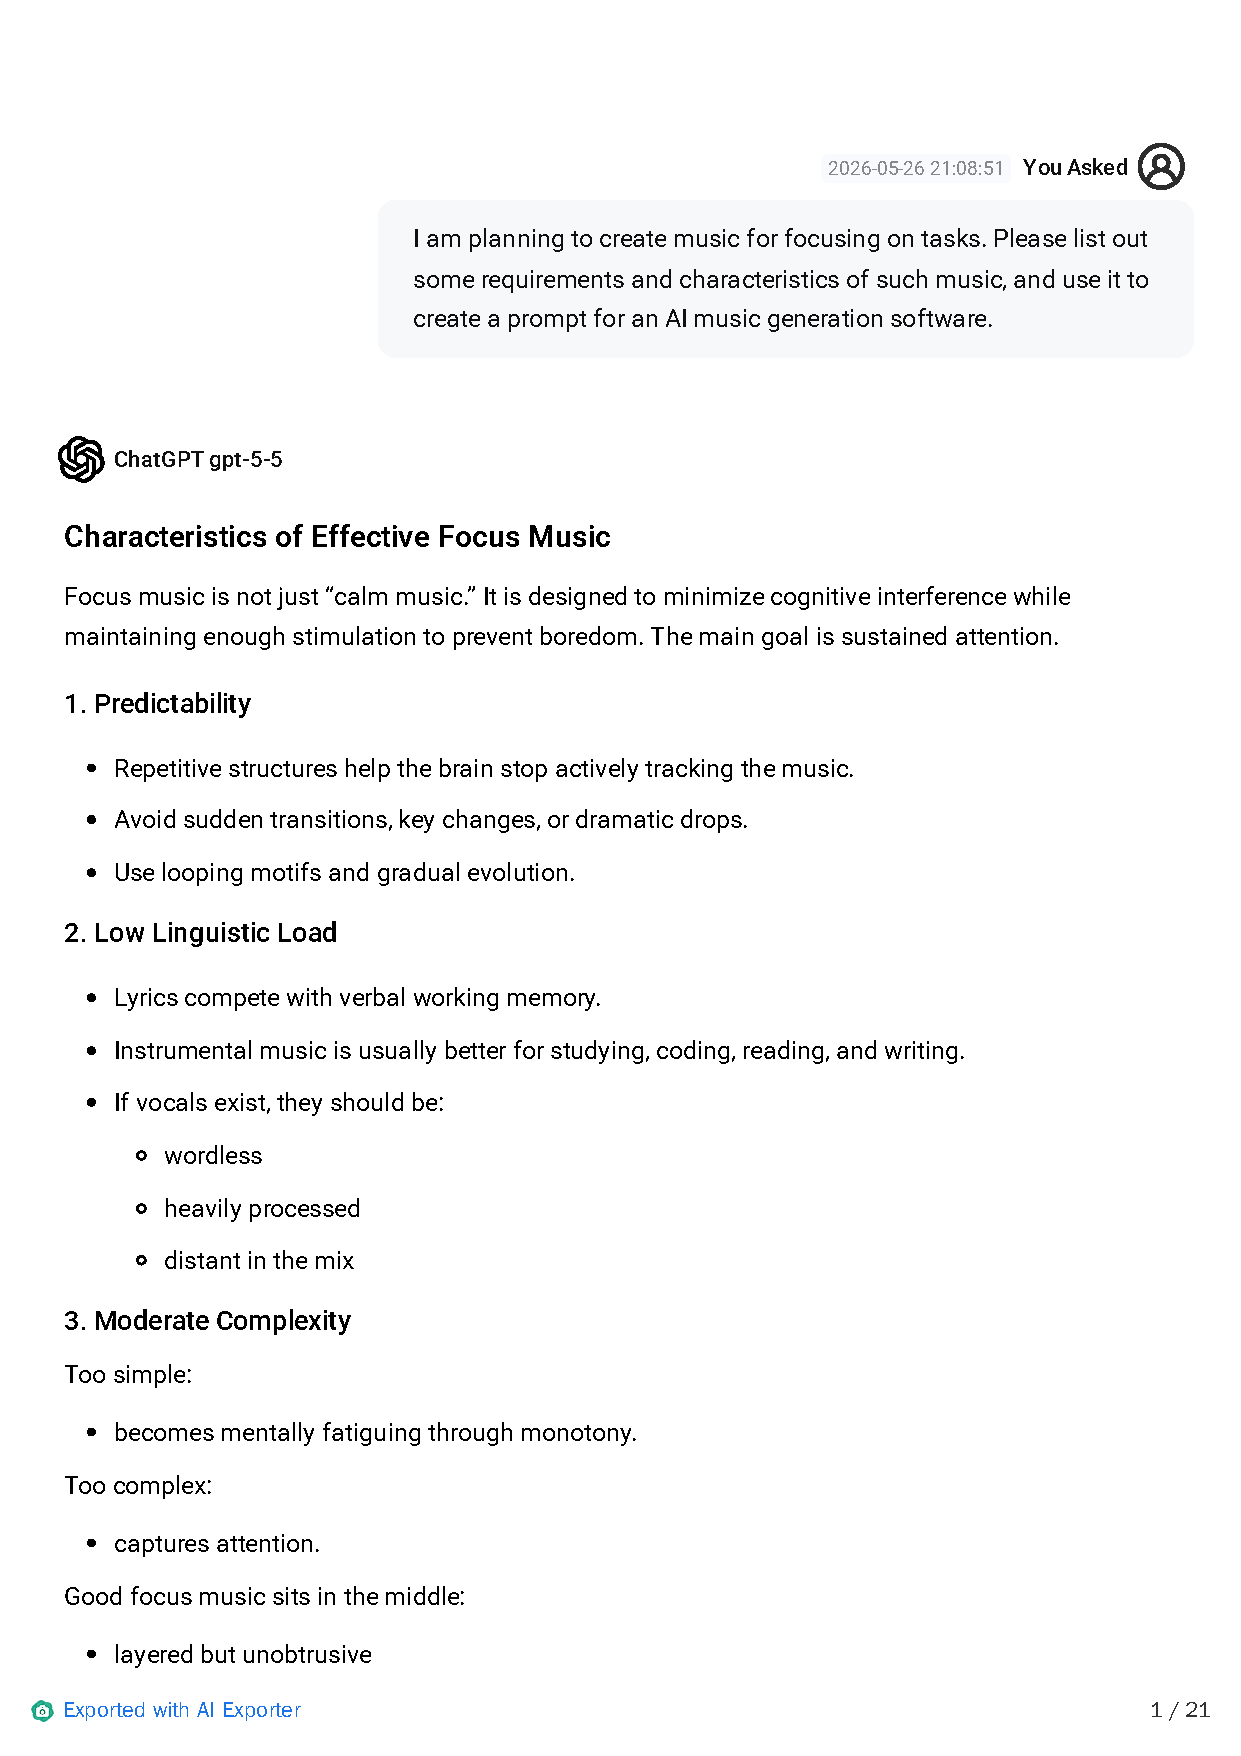
\includepdf[pages=-]{Focus Music Requirements.pdf}%
}{%
  \begin{center}
    \textit{（附录 PDF 文件 \texttt{Focus Music Requirements.pdf} 未包含在本仓库中；请将文件放入 \texttt{paper/} 目录后重新编译。）}
  \end{center}%
}

\end{document}
